% Copyright (c) 2026 JG Systems Consulting Ltd. See LICENSE.
% SPDX-License-Identifier: MIT
%
% Longer IEEE two-column preprint (~10 pages). The short practice cut is
% soam-ieee-software.tex (4 pages). Build: build-long.sh or build-long.ps1.

\documentclass[10pt,journal,compsoc]{IEEEtran}

\usepackage[T1]{fontenc}
\usepackage[utf8]{inputenc}
\usepackage{cite}
\usepackage{url}
\usepackage{booktabs}
\usepackage{tabularx}
\usepackage{xcolor}
\usepackage{tikz}
\usetikzlibrary{arrows.meta,positioning,shapes.geometric,fit,calc}
\usepackage[hidelinks]{hyperref}
\definecolor{soamfill}{gray}{0.94}
\definecolor{soamgate}{gray}{0.88}

\hyphenation{Archi-Mate Archi SOAM}

\begin{document}

\title{Keeping Architecture on Cadence: Skill-Orchestrated ArchiMate Modelling in the System of Record}

\author{JG~Systems~Consulting~Ltd%
\thanks{Preprint draft, not peer reviewed. Not an IEEE Software publication. Affiliation: JG Systems Consulting Ltd.}%
}

\markboth{Preprint (not peer reviewed)}{JG Systems Consulting Ltd: Skill-Orchestrated ArchiMate Modelling}

\IEEEtitleabstractindextext{%
\begin{abstract}
Delivery teams ship weekly. Architecture views lag by sprints. The lag is not a shortage of ArchiMate or of Archi: the modelling method lives in the architect's head and the tool is a canvas. Skill-Orchestrated ArchiMate Modelling (SOAM) is a governed pipeline: an orchestrator elicits intent and a view plan, the architect approves, then specialists write only into Archi through an MCP bridge. The ArchiMate language stays in MCP resources rather than in the agent. Two author-run frozen briefs demonstrate the pipeline: a mill CRM programme that must not absorb the MES (Hatherley Plate), and a training-range planning tool that must not absorb the GCS or the airborne computer (Moorfield Range). The defence is demonstration, not timing. The claim is method, not a speedup percentage.
\end{abstract}

\begin{IEEEkeywords}
enterprise architecture, ArchiMate, Archi, modelling tools, large language models, Model Context Protocol, human in the loop
\end{IEEEkeywords}}

\maketitle
\IEEEdisplaynontitleabstractindextext
\IEEEpeerreviewmaketitle

\section{Introduction}

Enterprise architecture is supposed to be the system of record for change. In an engineering organisation it often is not. In practice ArchiMate work is an unrecorded process. The architect runs a workshop, chooses a viewpoint without recording the choice, and places boxes in Archi for days. Review finds the wrong cut. The rationale ends up in slides the model never holds.

ISO/IEC/IEEE 42010 already said stakeholders get viewpoints~\cite{iso42010}. ArchiMate defined them~\cite{archimate32}. Archi holds a real model~\cite{archi}. The bottleneck is not the language: the method lives in the modeller's head and the tool is a canvas. Delivery teams ship weekly. Architecture views lag by sprints. That lag is a throughput problem: architecture cannot keep cadence with engineering because the method is uninstrumented. Throughput here is relevance, not a measured result. Skill-Orchestrated ArchiMate Modelling (SOAM) is the artefact offered against that problem: architect-governed, system-of-record native, and MCP-instrumented.

SOAM is a human-governed method: orchestrator-dispatched specialists for elicitation, viewpoint selection, layer modelling, traceability, quality assurance, layout, and documentation, writing only into Archi through an MCP bridge, with the ArchiMate language kept in MCP resources rather than in the agent~\cite{jgsarchiskills,jgsarchibridge,mcp2025}. Coding-agent hosts (ZCode, Claude Code) are runtime, not the artefact.

We do not claim that ArchiMate is incomplete, that TOGAF is the problem, or that architects are slow. Given ArchiMate and Archi, dominant practice does not instrument the method, so architecture cannot keep cadence with engineering. Language-model modelling papers mostly emit a parallel artefact~\cite{camara2023,fill2023}. EA suites are still mostly undriveable by an agent without forking the language into a prompt. SOAM attacks both gaps at once.

This paper is for staff engineers and delivery architects who know ArchiMate and have watched views fall behind the backlog. It is not a language tutorial. It accounts for why the method never made it into the tool, and one way to put it there without surrendering the gate.

Section~\ref{sec:practice} describes traditional ArchiMate work as an engineering organisation runs it. Section~\ref{sec:related} places SOAM against viewpoints, model quality, language-model modelling, and method engineering. Section~\ref{sec:method} states the method rules, pipeline, specialist contract, and MCP instrument. Section~\ref{sec:demo} maps waste classes to pipeline stages and walks two frozen briefs plus a refusal control. Section~\ref{sec:limits} covers adoption and threats to validity. Section~\ref{sec:takeaways} concludes.

\section{Traditional ArchiMate work in an engineering organisation}
\label{sec:practice}

A typical cycle in a shop that already owns Archi starts when a programme sponsor asks for ``the architecture'' of a change: a second CRM, a landing zone, a quote-to-cash cut. Someone books a workshop. Notes go into a document. An architect later reconstructs intent in Archi from those notes, last quarter's views, and memory of which relationships the language allows. Viewpoint choice is rarely written down. The first view that appears on a shared screen is often a kitchen sink: business actors, applications, and a node or two, because that is what fitted last time.

Review is late. Stakeholders see the drawing after the boxes exist. The wrong audience is found when the COO cannot find a capability cut and IT cannot find the integration. Rework is placing boxes again, not rerunning a method. Cross-layer traces (capability to process to application to node to work package) are the first labour dropped under a full programme week. Rationale, if it survives, lives in a slide that will not be opened when the model is next copied.

That loop is an uninstrumented method on a canvas tool. ArchiMate and 42010 already told the architect what a viewpoint is~\cite{iso42010,archimate32}. They did not put elicitation, viewpoint selection, correspondence, QA, layout, and documentation on a critical path the tool can run. Engineering organisations feel this as lag: delivery ships weekly; architecture views arrive a sprint later, or not at all, and the team proceeds on tribal knowledge.

Language-model assistants entered this gap as diagram generators. The failure mode is the opposite of the canvas problem. Generation is fast; the artefact is not the model. The architect is asked to approve a picture. Illegal relationships are a prompt accident. The Archi file operations and the next programme will open is unchanged~\cite{camara2023,fill2023}. The line has reached ArchiMate itself~\cite{nast2026}, and metamodel handling remains the weak point of prompt-carried language~\cite{muff2024}.

SOAM is an approach that neither adds drawing time nor produces a second artefact. It writes into Archi after a human gate, with the language left on the MCP.

\section{Related work}
\label{sec:related}

\subsection{Viewpoints and EA practice}

ISO/IEC/IEEE 42010 frames architecture description as stakeholders, concerns, viewpoints, and correspondence~\cite{iso42010}. ArchiMate supplies a layered language and a catalogue of viewpoints for those concerns~\cite{archimate32}. Lankhorst treats enterprise architecture as a working practice, not a drawing hobby~\cite{lankhorst2017}. Greefhorst and Proper put architecture principles at the centre of that practice~\cite{greefhorst2011}. Proper and Lankhorst argue that EA is essential sensemaking for the organisation~\cite{proper2014}. Jonkers et al.\ call the architecture both a management tool and a blueprint~\cite{jonkers2006}. TOGAF's Architecture Development Method, taken lightly, is a cycle of architecture work rather than a drawing task~\cite{togaf10}. Archi is the open-source toolkit where many practitioners place those views~\cite{archi}.

The language and the tool exist; the method still lives in the modeller's head. Viewpoint choice stays tacit; correspondence stays optional. A practitioner copies last week's view, fills an overloaded diagram, and finds the wrong audience in review. Nothing in 42010 or the ArchiMate specification executes that choice inside the tool.

\subsection{Model quality and correspondence}

Moody's physics of notations shows that visual languages fail as communication when graphic economy and cognitive load are ignored~\cite{moody2009}. Quartel et al.\ showed that goal-oriented motivation can be modelled in the EA stack rather than left in a separate requirements pile~\cite{quartel2009}. Hacks et al.\ named enterprise-architecture debt as the residue of postponed correspondence and quality work~\cite{hacks2019}. In ArchiMate practice the allowed-relationship table, completeness of traces, and layout of a view are the daily quality problems.

Checks and style guides run after the modelling: draw, check, then paste documentation into a slide. SOAM puts traceability, quality assurance, and layout on the critical path after layer modelling and before the run is treated as a draft.

\subsection{Language-model assisted modelling}

C{\'a}mara et al.\ assessed ChatGPT on UML modelling tasks and reported mixed reliability outside a controlled prompt~\cite{camara2023}. Fill, Fettke, and K{\"o}pke reported conceptual-modelling experiments in which models emit plausible diagrams that are not the organisation's model~\cite{fill2023}. Surveys cover the line: Di Rocco et al.\ map LLM use across model-driven engineering~\cite{dirrocco2025}, and a BISE editorial by Fill, Horkoff, Fettke, and K{\"o}pke names generative conceptual modelling a research direction~\cite{fill2026}. Nast et al.\ generate ArchiMate models from natural language~\cite{nast2026}; Chen and Zhao dispatch multiple agents on enterprise-architecture design~\cite{chen2024}. A growing set of papers generate PlantUML, JSON, or pictures from text. Some wrap a drawing tool. The Model Context Protocol is the open tool-and-resource interface those agents can speak~\cite{mcp2025,hou2025}. It is instrumentation, not a modelling method.

Those papers emit a parallel artefact. They copy or approximate the metamodel in the prompt. The system of record is unchanged. SOAM writes into Archi. Language source of truth stays in MCP resources. Architect approval of a view plan is a method rule, not a UI confirm on a generated picture.

\subsection{Design science and method engineering}

Hevner et al.\ locate design-science contributions in artefacts evaluated against a problem~\cite{hevner2004}. Peffers et al.\ license demonstration plus informed argument as evaluation for a first method paper~\cite{peffers2007}. Brinkkemper defined method engineering as the engineering of methods and tools~\cite{brinkkemper1996}. Ralyt{\'e}, Deneck{\`e}re, and Rolland treat situational method engineering as composition of fragments under a situation~\cite{ralyte2003}.

Design science licenses demonstration plus informed argument. Situational method engineering treats fragments and composition. Neither supplies an architect-governed, system-of-record-native modelling pipeline. SOAM uses specialists as method fragments and the orchestrator as composition. This paper is not an SME treatise. The evaluation demonstrates that those fragments can be dispatched against named waste classes, with the architect still on the gate.

Table~\ref{tab:compare} is the comparison an engineer needs. Traditional ArchiMate practice keeps the system of record and loses the method. Language-model diagram generation keeps a method-shaped prompt and loses the system of record. SOAM keeps both.

\begin{table*}[!t]
\caption{Where the model lives, who governs, and what the language source of truth is.}
\label{tab:compare}
\centering
{\small
\begin{tabularx}{\textwidth}{@{}>{\raggedright\arraybackslash}p{0.16\textwidth} *{3}{>{\raggedright\arraybackslash}X}@{}}
\toprule
 & \textbf{Traditional Archi practice} & \textbf{LLM diagram generation} & \textbf{SOAM} \\
\midrule
System of record & Archi, if the architect finishes & Parallel PlantUML, JSON, or picture & Archi, written through MCP \\
Viewpoint choice & Tacit; last week's view & Prompt or overloaded diagram & Viewpoint-select, then approval \\
When written & After workshops, over days & Immediately, outside Archi & After view-plan approval \\
Language SoT & Spec on the shelf & Copied into the prompt & MCP resources \\
Correspondence & Optional labour & Rarely a stage & Traceability on the critical path \\
Documentation & Slide deck & Caption on the picture & Fields on the elements \\
Architect authority & High, slow & Low, after the fact & High, as a gate before mutate \\
\bottomrule
\end{tabularx}}
\end{table*}

\section{Skill-Orchestrated ArchiMate Modelling}
\label{sec:method}

SOAM is a method: an orchestrator, twelve specialists, and a consume-only MCP bridge into Archi~\cite{jgsarchiskills,jgsarchibridge}. The language is not in the skills.

\subsection{Five rules}

\begin{enumerate}
\item \textbf{The user governs.} Input is plain-language intent. Specialists do not mutate until the architect approves a view plan naming views, stakeholders, concerns, and layer specialists. Scope refusals are method behaviour. A refused redesign is not a failed generation. The architect can reject and return to elicitation with no half-written model.

\item \textbf{The orchestrator composes; specialists execute.} Elicitation and viewpoint selection run first; only named layers are dispatched; the user does not invoke layer skills. That rule stops modelling every layer: a capability cut does not silently grow a technology view, and a landing-zone move does not invent a new operating model to justify the diagram.

\item \textbf{Archi is the only canvas.} Elements, relations, views, and documentation fields are written through MCP. No parallel diagram. No PlantUML as the deliverable. The model the organisation already keeps is the model the run writes. Inspect-before-create is part of the shared contract: specialists re-query identifiers, reuse existing elements where names match, and surface ambiguous near-matches instead of silent merges.

\item \textbf{The language stays in MCP resources.} Skills orchestrate tools and resources and do not embed the ArchiMate metamodel, which current models handle unreliably~\cite{muff2024}. A structural check stops a skill citing a tool absent from the bridge. Allowed relationships, viewpoint definitions, and recipes stay on the MCP. If the language changes in Archi, skills do not carry a stale copy.

\item \textbf{Correspondence is a stage.} Traceability runs after layer specialists; quality assurance, layout, and documentation are terminal. Every created element carries an evidence line (stated, inferred, or existing) in its documentation field. Rationale lives in the model, not in a second artefact. The documentation specialist ends at a draft checkpoint; the first generation is not presented as finished work.
\end{enumerate}

A prompt that says ``draw ArchiMate'' has none of these rules.

\subsection{Pipeline}

Fig.~\ref{fig:pipeline} shows the run: elicit intent, draft viewpoint selection, gate on the view plan; rejection returns to intent; approval dispatches only named layer specialists, then traceability, model QA, layout, and documentation.

\begin{figure}[!t]
\centering
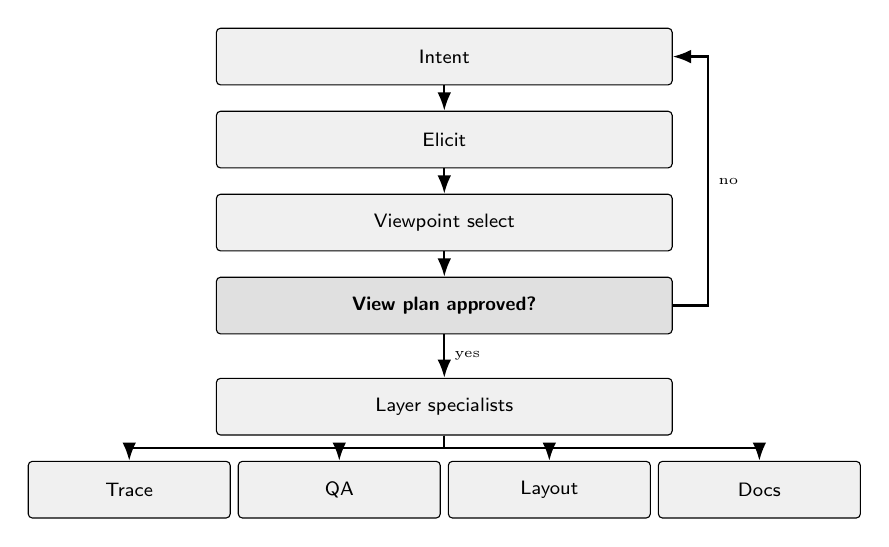
\begin{tikzpicture}[
  font=\sffamily\scriptsize,
  box/.style={draw, rounded corners=1.5pt, align=center, inner sep=3pt,
    minimum height=7.2mm, text width=0.46\columnwidth, fill=soamfill},
  gate/.style={draw, rounded corners=1.5pt, align=center, inner sep=3pt,
    minimum height=7.2mm, text width=0.46\columnwidth, fill=soamgate,
    font=\sffamily\scriptsize\bfseries},
  sm/.style={draw, rounded corners=1.5pt, align=center, inner sep=2pt,
    minimum height=7.2mm, text width=0.20\columnwidth, fill=soamfill},
  arr/.style={-{Latex}, thick}
]
\node[box] (I) {Intent};
\node[box, below=3.2mm of I] (E) {Elicit};
\node[box, below=3.2mm of E] (V) {Viewpoint select};
\node[gate, below=3.2mm of V] (A) {View plan approved?};
\node[box, below=5.5mm of A] (L) {Layer specialists};
\node[sm, below=3.2mm of L, xshift=-0.33\columnwidth] (T) {Trace};
\node[sm, below=3.2mm of L, xshift=-0.11\columnwidth] (Q) {QA};
\node[sm, below=3.2mm of L, xshift=0.11\columnwidth] (Y) {Layout};
\node[sm, below=3.2mm of L, xshift=0.33\columnwidth] (D) {Docs};
\draw[arr] (I) -- (E);
\draw[arr] (E) -- (V);
\draw[arr] (V) -- (A);
\draw[arr] (A) -- node[right, font=\tiny] {yes} (L);
\draw[arr] (L.south) -- ++(0,-1.6mm) -| (T.north);
\draw[arr] (L.south) -- ++(0,-1.6mm) -| (Q.north);
\draw[arr] (L.south) -- ++(0,-1.6mm) -| (Y.north);
\draw[arr] (L.south) -- ++(0,-1.6mm) -| (D.north);
\draw[arr] (A.east) -- ++(4.5mm,0) |- node[pos=0.25, right, font=\tiny] {no} (I.east);
\end{tikzpicture}
\caption{SOAM pipeline. Nothing mutates until the view plan is approved. Trace, QA, layout, and documentation run after the named layer specialists.}
\label{fig:pipeline}
\end{figure}

Layer specialists: motivation, capability and strategy, business, application, technology and physical, implementation and migration. The mill CRM brief includes motivation plus technology and physical, and omits implementation and migration. The range brief does the same and also refuses SysML and an air-vehicle product structure. Dispatch follows the plan, not a default of every layer.

\subsection{Specialists}

The user invokes only the orchestrator. The orchestrator dispatches the specialists in Table~\ref{tab:specialists}. A thirteenth skill in the published pack files pack defects; it is not part of SOAM and is out of this paper.

\begin{table}[!t]
\caption{Orchestrator-dispatched specialists. Mutations only after view-plan approval.}
\label{tab:specialists}
\centering
{\scriptsize
\begin{tabularx}{\columnwidth}{@{}>{\raggedright\arraybackslash}p{0.30\columnwidth} >{\centering\arraybackslash}p{0.14\columnwidth} >{\raggedright\arraybackslash}X@{}}
\toprule
\textbf{Specialist} & \textbf{Mutates} & \textbf{Job} \\
\midrule
elicit & no & Normalise intent \\
viewpoint-select & no & Ground viewpoint to stakeholder and concern \\
motivation & yes & Drivers, goals, outcomes \\
capability / strategy & yes & Capabilities and resources \\
business & yes & Actors, processes, services \\
application & yes & Components and data objects \\
technology / physical & yes & Nodes, facilities, equipment \\
impl./migration & yes & Plateaus, gaps, work packages \\
traceability & yes & Cross-layer relations still open \\
model-qa & report first & Compliance; fixes only if approved \\
layout & yes & Archi-native layout on existing views \\
documentation & yes & Rationale fields; draft summary \\
\bottomrule
\end{tabularx}}
\end{table}

\subsection{Shared modelling contract}

The shared contract (CREATE\_PATH) keeps twelve specialists from forking twelve create paths. Two gates are binding in prose here.

CP-G1, confirm-before-mutate: no mutating MCP call unless the view plan is approved. Without this gate the pipeline is a generator behind a chat UI.

CP-G7, first generation is a draft: the documentation specialist ends at a draft checkpoint. Completing a specialist does not finish the model.

Table~\ref{tab:gates} lists the contract gates. They exist because agent runs fail in ordinary ways: stale identifiers after context compaction, silent skips in a hand-off, invented elements with no source, notes placed before layout is closed, and a specialist announcing the model finished because its own work ended.

\begin{table}[!t]
\caption{Shared modelling-contract gates (CREATE\_PATH).}
\label{tab:gates}
\centering
{\scriptsize
\begin{tabularx}{\columnwidth}{@{}l >{\raggedright\arraybackslash}p{0.26\columnwidth} >{\raggedright\arraybackslash}X@{}}
\toprule
\textbf{ID} & \textbf{Gate} & \textbf{Pass} \\
\midrule
CP-G1 & Confirm-before-mutate & No mutate until the view plan is approved \\
CP-G2 & Fresh IDs & Re-query IDs at start and after compaction \\
CP-G3 & Disposition complete & Every candidate captured, folded, needs-user, or out-of-scope \\
CP-G4 & No invention & Evidence line: stated, inferred, or existing \\
CP-G5 & Annotate last & Notes and legends last on the view \\
CP-G6 & Render close-out & Layout check, then inspect an exported view \\
CP-G7 & First generation is a draft & Documentation ends at a draft checkpoint \\
\bottomrule
\end{tabularx}}
\end{table}

These are method integrity rules, not a quality experiment. CP-G1 and CP-G7 are the ones that change organisational behaviour: nothing is written without approval, and the first generation is not finished work.

\subsection{MCP as instrument}

The JGS Archi Bridge runs inside Archi and exposes HTTP MCP at \texttt{http://127.0.0.1:18090/mcp} by default~\cite{mcp2025,hou2025,jgsarchibridge}. Offline inventory: 69 tools, 14 resources. Skills consume those only; they never modify the bridge or copy ArchiMate language tables into skill text. They read \texttt{archimate://reference/*} and \texttt{archimate://recipes/*} from the MCP. Archi 5.7 or later is the modelling surface~\cite{archi,jgsarchiskills}.

MCP makes the system of record agent-operable~\cite{mcp2025}. SOAM supplies the method on that surface. If the paper led with MCP, it would be a protocol note. Engineers should care about the gate and the canvas, not the port number.

\subsection{Implementation}

jgs-archi-skills v1.0.0 is MIT~\cite{jgsarchiskills}. JGS Archi Bridge is the consume-only partner~\cite{jgsarchibridge}. Helpers are Python 3.10 standard-library validators (viewpoint matrices, compliance asserts, structural checks), not a modelling engine. Skills are stateless. Model content and rationale live in Archi documentation fields. The repo holds skills, helpers, and tests. Live MCP is an opt-in smoke path, not evidence for this article.

The implementation is a method, not a prompt pack, for four choices already stated: the approval gate, specialist dispatch as fragments, the consume-only language contract, and the waste-class mapping in Section~\ref{sec:demo}.

From the architect's chair, the architect types plain-language intent into the orchestrator, not an element-type command. Elicit normalises stakeholders, concerns, scope in, and scope out. Viewpoint-select proposes views and names the specialists those views need. The orchestrator stops. The architect reads the view plan. Approval is the only thing that opens MCP mutate. Specialists then write into the open Archi model, reuse existing elements where names match, and leave traces, a QA report, a layout pass, and documentation fields. The documentation specialist stops at a draft. The architect still owns whether that draft is the architecture or a first cut to discard.

That is the cadence claim in operational form. The workshop, the unrecorded viewpoint, the week of boxes, and the late review are replaced by a gated pipeline that still cannot write without approval.

The view plan the architect is asked to sign is not a diagram. It is a short contract: intent restated, stakeholders and concerns, scope in and scope out, named views, named specialists, and the constraints the run must not violate (OrderSight stays distinct from MillOS; RangePlan stays distinct from GroundOS and AirStack; no SysML on this canvas). If that contract is wrong, the architect rejects it. Nothing has been written yet. That is cheaper than finding the wrong cut after fifty boxes exist.

Fig.~\ref{fig:plan} is the shape of that contract for the mill CRM brief. It sketches the fields; it is not a log of a live run.

\begin{figure}[!t]
\centering
{\small
\begin{tabularx}{\columnwidth}{@{}>{\bfseries\raggedright\arraybackslash}p{0.28\columnwidth} >{\raggedright\arraybackslash}X@{}}
\toprule
Intent & Mill as-is plus CRM for order visibility \\
Stakeholders & Plant manager, sales, MES owner, CRM programme \\
In & Motivation, capabilities, operations, apps, tech, mill equipment \\
Out & Work packages, costing, MES rewrite \\
Views & Motivation Overview; Capability Map; Production Operations; Application Support; Technology and Physical \\
Specialists & Motivation, capability, business, application, technology-physical, then trace, QA, layout, docs \\
Constraints & OrderSight stays distinct from MillOS; equipment on a node; no roadmap \\
Gate & Approved or rejected (nothing written until yes) \\
\bottomrule
\end{tabularx}}
\caption{View-plan fields for the mill CRM brief. Approval opens MCP mutate. Rejection writes nothing.}
\label{fig:plan}
\end{figure}

\subsection{What the three briefs dispatch}

Table~\ref{tab:briefs} puts the situational part of the method in one place. The mill CRM never calls implementation-migration. The range brief matches that cut and also refuses SysML and an air-vehicle product structure. The orchestrator does method composition, not template fill.

\begin{table*}[!t]
\caption{Frozen briefs, views, specialists, and the constraint that would fail the run.}
\label{tab:briefs}
\centering
{\small
\begin{tabularx}{\textwidth}{@{}>{\raggedright\arraybackslash}p{0.18\textwidth} >{\raggedright\arraybackslash}p{0.26\textwidth} >{\raggedright\arraybackslash}p{0.26\textwidth} >{\raggedright\arraybackslash}X@{}}
\toprule
\textbf{Brief} & \textbf{Views} & \textbf{Layer specialists} & \textbf{Hard constraint} \\
\midrule
Hatherley Plate & Motivation; Capability Map; Production Operations; Application Support; Technology and Physical & motivation, capability, business, application, technology-physical & OrderSight distinct from MillOS; equipment on a node; no roadmap \\
Moorfield Range & Motivation; Capability Map; Range Operations; Application Support; Technology and Physical & motivation, capability, business, application, technology-physical & RangePlan, GroundOS, AirStack distinct; no SysML; air vehicle not product structure \\
\bottomrule
\end{tabularx}}
\end{table*}

\section{Demonstration}
\label{sec:demo}

Evaluation follows Peffers: demonstration plus informed argument~\cite{peffers2007}. A reviewer should finish this section able to replay both walks and see each waste class hit by a named stage. Both walks were executed by the authors in Archi 5.7+ through the JGS Archi Bridge. Neither is a timed client engagement. Working models live in \url{https://github.com/jgsystemsconsulting/jgs-archi-skills-we}.

\subsection{Waste classes and stages}

Table~\ref{tab:waste} lists recurring cycle-time waste. Each row names the SOAM stage built for that waste.

\begin{table}[!t]
\caption{Tool-as-canvas waste and the pipeline stage that addresses it.}
\label{tab:waste}
\centering
{\scriptsize
\begin{tabularx}{\columnwidth}{@{}>{\raggedright\arraybackslash}p{0.28\columnwidth} >{\raggedright\arraybackslash}X >{\raggedright\arraybackslash}p{0.30\columnwidth}@{}}
\toprule
\textbf{Waste} & \textbf{What it costs} & \textbf{SOAM stage} \\
\midrule
Viewpoint chosen from habit or last week's view & Wrong audience, overloaded diagrams, rework & Viewpoint-select and view-plan approval \\
Elicitation and modelling decoupled & Notes go stale; review finds the wrong scope & Elicit, then plan; no mutate yet \\
Drawing labour as the main effort & Consistency and allowed relations stay in the modeller's head & Layer specialists via MCP \\
Cross-layer correspondence optional & Motivation to capability to application to technology to work package breaks first under deadline & Traceability \\
Documentation as a second artefact & Rationale in slides; model becomes a picture archive & Documentation fields in the model \\
Language knowledge not executable & Junior staff invent illegal relations; seniors lint & MCP resources and model-qa \\
\bottomrule
\end{tabularx}}
\end{table}

SOAM runs elicit, plan, model, QA, and document as one governed run. Table~\ref{tab:waste} supports the cycle-time claim. No timing was done.

\subsection{Walk A: Hatherley Plate}

Hatherley Plate is a UK plate mill. Production runs on MillOS (MES) and WorksERP; sales still track promises on PromiseSheet. OrderSight is funded for order visibility. Plant engineers worry OrderSight will be drawn as if it replaces MillOS. Stakeholders: plant manager, head of sales, MES owner, CRM programme manager, operations planner, integration lead. Concerns: order visibility from promise to mill schedule; OrderSight must not absorb MillOS; equipment and the mill building stay in scope; what PlantGate connects. Scope in: motivation for visibility, capabilities, production operations, applications, technology nodes, physical equipment or facility. Scope out: work-package roadmap, product costing, greenfield MES rewrite. Current state: MillOS schedules the mill; WorksERP holds works orders; PromiseSheet holds customer promises; OrderSight is in pilot; PlantGate sits in the plant comms room. Target: mill equipment and MillOS still visible; OrderSight sales-facing, served by PlantGate; shared order identity, not one merged blob.

Views: Motivation Overview, Capability Map, Production Operations, Application Support, Technology and Physical. Specialists: elicit, viewpoint-select, motivation, capability-strategy, business, application, technology-physical, traceability, model-qa, layout, documentation. Pass checks: listed views; OrderSight and MillOS remain separate applications; WorksERP, PromiseSheet, and PlantGate stay distinct; at least one facility or equipment element on a mill-floor node; confirmation gate before mutate.

This is the engineering-organisation case: a funded programme collides with mill operations. Sales wants order visibility. The mill already has a MES that schedules production and an ERP that holds works orders. If an architect or agent draws OrderSight as the system that runs the mill, the model would be used against the plant. The method must keep OrderSight and MillOS separate, keep mill equipment on a node, and still show PlantGate in the comms room connecting sales-facing identity to works orders. Pictures of the five views sit on \texttt{hatherley.html}. Author-run frozen firm, not a client model.

Motivation is in for visibility; technology and physical are in for mill equipment and PlantGate; implementation and migration are out because the brief forbids a work-package roadmap. The hard constraints are method tests: if OrderSight absorbs MillOS on the canvas, the run failed even if the diagram has many elements. Correspondence here is equipment assigned to a node and refusal to merge two applications the plant does not treat as one. Modelling every layer would add a migration plateau the brief excluded. Dispatch keeps that plateau off the plan.

\subsection{Walk B: Moorfield Range}

Hawker Range Systems Ltd runs one UK training range at Moorfield. Instructors still track sorties on SortieBoard. RangePlan is funded for sortie visibility. The plant analogue: RangePlan must not be drawn as GroundOS (GCS software) or as AirStack (airborne mission computer). Stakeholders: range manager, chief instructor, GCS owner, planning programme manager, sortie planner, integration lead. Concerns: sortie visibility from tasking to live GCS; RangePlan must not absorb GroundOS or AirStack; hangar, GCS van, and range equipment stay in scope; what LinkGate connects. Scope in: motivation for visibility, capabilities, range operations, applications, technology nodes, physical equipment or facility. Scope out: work-package roadmap, second site, GroundOS rewrite, weapons, ERP, air-vehicle SysML. Current state: GroundOS owns the live sortie; AirStack is the airborne mission computer; SortieBoard is the day's spreadsheet; RangePlan is in pilot; LinkGate sits in the comms cabin. Target: RangePlan, GroundOS, and AirStack stay separate; shared sortie identity, not one merged blob; LinkGate bridges tasking to GroundOS and does not talk to the air vehicle.

Views: Motivation Overview, Capability Map, Range Operations, Application Support, Technology and Physical. Specialists match the mill cut: motivation and technology-physical in; implementation and migration out. Pass checks: listed views; RangePlan, GroundOS, and AirStack remain separate applications; at least one facility or equipment element on a node; air vehicle not modelled as product structure; SysML stays off this canvas; confirmation gate before mutate.

Moorfield is the refuse-scope walk the paper still needs: dispatch does not invent SysML, a work-package plateau, or a merged blob. Pictures are not on \texttt{hatherley.html}; the working model is in the same we-repo named in the demonstration opener. Author-run frozen firm, not a client model. Without this control, SOAM acts as a generator that always fills every layer and every neighbouring notation.

\subsection{Method integrity}

A structural validator in the skill pack (\texttt{helpers/validate\_skill\_mcp\_refs.py}) checks skill files cite only tools and resources in the bridge inventory. On the v1.0.0 pack it reports fourteen skill files and zero unknown references. That warrants the tool-cite claim, not modelling quality.

The copy-free language contract is a consume-only policy, not a validator result: skills consume MCP tools and resources only and never copy ArchiMate language tables into skills; they read \texttt{archimate://reference/*} and \texttt{archimate://recipes/*} from the MCP. Confirm-before-mutate remains CP-G1. These are integrity properties of the implementation, not an experiment on diagram quality.

\section{Limits and adoption}
\label{sec:limits}

SOAM is built so a shop that already runs Archi can install it: MIT skills, no second EA suite, architect on the gate. That is a design choice for industry uptake, not evidence that industry has taken the method up. Treating design-for-adoption as a finding would overstate the evidence.

Both walks are author-run Archi models, not client engagements. They show method coverage, not organisational uptake. Starter prompts for invoice-to-cash and a landing-zone refuse exist in the skill pack and are not this paper's evidence. The implementation is one bridge, one skill suite, Archi only; the argument does not generalise to Sparx or LeanIX. Language-model output is non-deterministic: the same intent can yield different element names. Governance (approval gate, QA, no-invention rule) is the control, not model temperature. Assistant users over-trust output when verification is left to them~\cite{perry2023}. Hallucination is a standing failure mode of language models~\cite{ji2023}. The walks are by the method authors; this is demonstration, not an independent trial. Throughput is unmeasured. Adjacent measured evidence: a randomised GitHub Copilot trial completed coding tasks 55.8 percent faster~\cite{peng2023}. That number is about coding, not modelling. The cycle-time claim is reasoned from waste removal in Table~\ref{tab:waste}.

A later study should time hand modelling against SOAM on the same brief with a second architect, report one anonymised client run, measure whether repeated runs keep the same element names and view titles, and check whether QA reports the same defect classes a senior architect would. Those are future measurements, not results.

Table~\ref{tab:threats} restates those limits in one place.

\begin{table}[!t]
\caption{Threats to validity for this demonstration.}
\label{tab:threats}
\centering
{\scriptsize
\begin{tabularx}{\columnwidth}{@{}>{\raggedright\arraybackslash}p{0.28\columnwidth} X@{}}
\toprule
\textbf{Threat} & \textbf{What it means} \\
\midrule
Lab scenarios & Both walks author-run, not client. Starter prompts for invoice-to-cash and landing-zone refuse are pack copy, not evidence. Coverage, not uptake. \\
Single implementation & One bridge, one skill suite, Archi only. Not Sparx, not LeanIX. \\
LLM non-determinism & Same intent can yield different element names. Governance is the control, not temperature. \\
Author as evaluator & Walks are by the method authors. Demonstration, not an independent trial. \\
Throughput unmeasured & Cycle-time claim is reasoned from Table~\ref{tab:waste}. No timing was done. \\
\bottomrule
\end{tabularx}}
\end{table}

Until that study exists, an engineering organisation can still decide whether to install the method. The test is local: open Archi, start the bridge, install the skills, run one frozen brief against a throwaway model, and ask whether the view plan is something an architect would sign. If the plan is not worth signing, the method failed before any box was placed. That is the point of the gate.

A trial worth doing in a week: pick one live change already in the backlog, not a greenfield scenario. Run SOAM against a copy of the current Archi model. Keep the original model closed. Compare the view plan to what the architect would have drawn by hand: named views, named exclusions, named constraints. Then look at correspondence. If the pipeline cannot keep OrderSight distinct from MillOS on a plant brief, or merges RangePlan into GroundOS on a range brief, stop. Those are method failures, not taste. If the plan is signable and the constraints hold, the remaining question is labour: how long the gated run took versus the last time this team modelled a similar cut. That comparison is the follow-up paper, not this one.

\section{Takeaways}
\label{sec:takeaways}

\begin{itemize}
\item SOAM is a human-governed method that dispatches specialists after an approved view plan, not a prompt pack that draws diagrams.
\item The system of record stays Archi; the ArchiMate language stays in MCP resources; the agent does not fork the metamodel.
\item Instrument the method in the model you already keep. Put the architect on a view-plan gate before any mutate. Treat missing traces, missing layout, and slide-deck rationale as pipeline failures, not cleanup.
\item Cadence of architecture work is why an engineering organisation should care. Throughput is a relevance argument from removed waste classes, not a timed finding. Measure it later. Do not invent a percentage now.
\end{itemize}

\bibliographystyle{IEEEtran}
\bibliography{soam}

\end{document}
